\chapter{Collaboration Layer}
\label{chapter:collaborationlayer}

The collaboration layer is in between the two other layers: the network 
layer below and the application layer above. It is responsible for all the 
collaboration functionality. The core responsibilities are:

\begin{itemize}
 \item host the concurrency control algorithm
 \item transform incoming as well as outgoing requests
 \item manage the set of participants in a given session
 \item access control
\end{itemize}

The concurrency control algorithm is based on the concept of operational 
transformation. It was developed and tested as part of the semester project.
In the diploma project, the main task in this layer was to integrate the
algorithm into the layer design.

The collaboration layer can basically be split into two different parts: the
client part and the server part.



\section{CollaborationService}
The core entry point into the collaboration layer is the 
\texttt{Collaboration\-Service}. This interface is implemented by the
\texttt{Collaboration\-Service\-Impl} class, which also implements the
\texttt{Network\-Service\-Callback} interface. These interfaces and their
functionality have been thorougly explained before (see chapter 
\ref{chapter:archoverview}. The implementation passes the calls on 
the \texttt{Network\-Service\-Callback} methods to the corresponding
methods of the API between the collaboration and the application
layer.


\subsection{User and Document Management}
The collaboration service implementation delegates the management of the
set of currently discovered users and documents to objects implementing
\texttt{UserRegistry} and \texttt{DocumentRegistry} respectively.

The collaboration layer makes sure that for each unique user id there is
only one \texttt{RemoteUser}. Thus it is save to register a 
\texttt{PropertyChangeListener} on the \texttt{RemoteUser} to receive changes
to that user's name. It takes also care that there is only one 
\texttt{RemoteDocument} for a unique document id.

The \texttt{UserRegistry} manages the currently known set of users. The
objects registered in the registry are of type \texttt{MutableRemoteUser},
which adds a single method \texttt{setName} to the \texttt{RemoteUser}
interface. This method allows the collaboration layer to change the
name of a user, if such a change is reported from the network layer.
The \texttt{getUser} method with an argument of type
\texttt{RemoteUserProxy} creates a new \texttt{MutableRemoteUser}, if 
a user with the same id does not already exist. This makes sure that
there is only one \texttt{RemoteUser} object for a unique user. The
other \texttt{getUser} method returns null if there is no user in the
registry with the given id.

\begin{figure}[H]
 \centering
 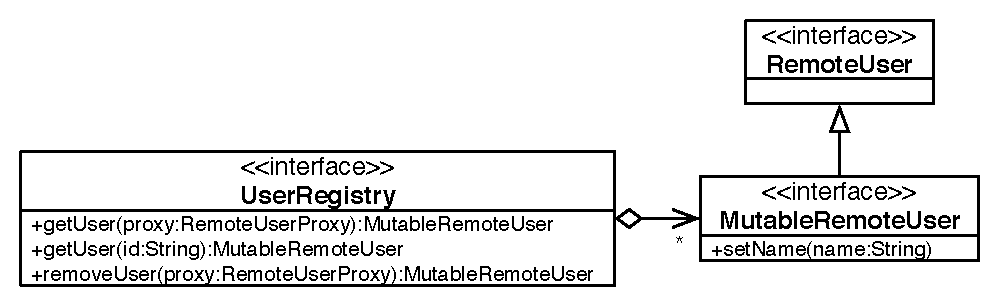
\includegraphics[width=16.37cm,height=4.62cm]{../images/finalreport/collaboration_userregistry_uml.eps}
 \caption{UserRegistry Interface}
 \label{fig:collaboration.userregistry}
\end{figure}

The \texttt{Document\-Registry} is the equivalent class for 
\texttt{Mutable\-Remote\-Document} objects. \texttt{Mutable\-Remote\-Document}
adds the \texttt{setTitle} method to the \texttt{RemoteDocument}.

\begin{figure}[H]
 \centering
 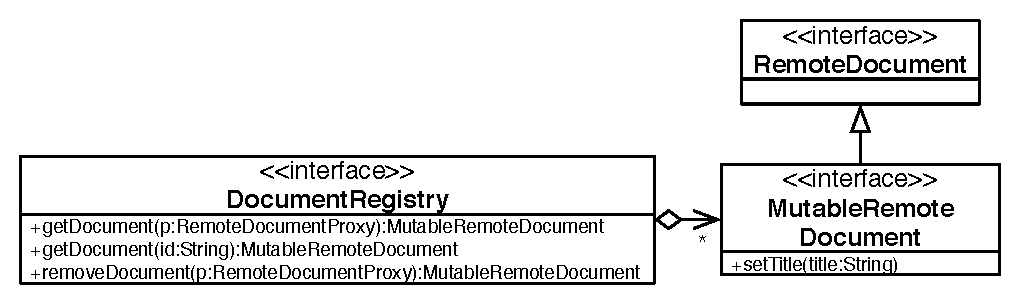
\includegraphics[width=16.72cm,height=4.59cm]{../images/finalreport/collaboration_documentregistry_uml.eps}
 \caption{DocumentRegistry Interface}
 \label{fig:collaboration.documentregistry}
\end{figure}

The mutable subinterfaces of \texttt{RemoteUser} and \texttt{RemoteDocument}
are passed to the application layer, because the user is never allowed to
change the name of other users or the title of documents published by other
users.



\section{Client Side}
The collaboration layer has to implement several interfaces defined in
the API to the adjacent layers.


\subsection{Receiving Invitations}
The collaboration layer has to implement the \texttt{Invitation} interface.
It is implemented by the \texttt{InvitationImpl} class. The implementation
is straightforward. The calls to \texttt{reject} and \texttt{accept} are
directly forwarded to the referenced \texttt{InvitationProxy} from the
network layer. The only thing the collaboration layer does is to wrap the
passed in \texttt{JoinCallback} with an implementation of 
\texttt{JoinNetworkCallback}.


\subsection{Join Callback}
To forward a join request to the network layer, the collaboration layer has
to implement the \texttt{JoinNetworkCallback} interface. The
\texttt{accepted} method of the interface must create a \texttt{Session}
and pass that to the \texttt{JoinCallback} of the application layer.
The callback must also return a \texttt{SessionConnectionCallback} to the
network layer.


\subsection{Creating Sessions}
\texttt{Session} objects are created by a \texttt{SessionFactory}. The
\texttt{SessionFactory} creates \texttt{ConfigurableSession} objects, which
provide methods to set the \texttt{SessionConnection} as well as the
\texttt{ParticipantSessionCallback}.


\subsection{Session Implementation}
The default implementation for the \texttt{Session} interface is the
\texttt{SessionImpl} class. It implements the \texttt{ConfigurableSession}
interface, which also implements the \texttt{SessionConnectionCallback}
interface. So the implementation acts as both the \texttt{Session} to
the application layer as well as \texttt{SessionConnectionCallback} to the
network layer.

\subsubsection{Transformations}
The \texttt{SessionImpl} class hosts the client-side transformation algorithm.
Every received request is transformed with that algorithm. Before a
received request can be transformed, the session has to be locked (locking
the lock passed from the application layer by the \texttt{getLock} method
of the \texttt{SessionCallback}). When sending operations, the algorithm
creates a request that can then be sent to the \texttt{SessionConnection}.

\subsubsection{Session Connection}
The \texttt{Configurable\-Session} has a method called \texttt{setConnection},
which passes the \texttt{Session\-Connection} to the \texttt{Session}. The
\texttt{Session\-Impl} makes use of a \texttt{Thread\-Domain} (see
chapter \ref{chapter:threaddomains}) to execute calls on the 
\texttt{SessionConnection} asynchronously. The main reason for doing this
is that the caller thread (most likely the AWT event dispatch thread)
is by a potentially slow network connection. The caller thread can go
on and execute other tasks.

However, using asynchronous calls has one significant
disadvantage. Exceptions thrown by the method invocation cannot be
thrown back at the caller (i.e. the application layer). That is where
the \texttt{SessionConnectionWrapper} helps out. It is an implementation
of the \texttt{SessionConnection} interface that catches all exceptions
thrown by the target \texttt{SessionConnection} and passes them to an
object implementing the \texttt{Session\-Connection.Failure\-Handler}
interface. The figure \ref{fig:collaboration.sessionconnectionwrapper}
shows exactly the described setup.

\begin{figure}[H]
 \centering
 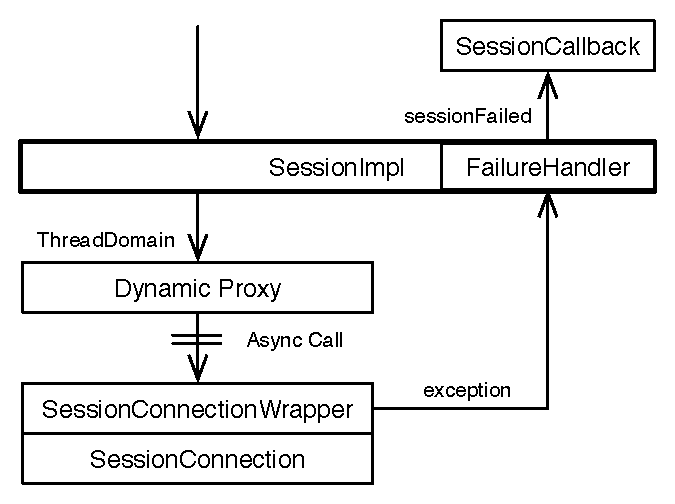
\includegraphics[width=10.87cm,9.28cm]{../images/finalreport/collaboration_sessionconnectionwrapper.eps}
 \caption{Wrapped session connection with ThreadDomains}
 \label{fig:collaboration.sessionconnectionwrapper}
\end{figure}

The call from the dynamic proxy to the \texttt{Session\-Connection\-Wrapper}
is asynchronous. The methods of the \texttt{Session\-Connection\-Wrapper}
are executed by a designated worker thread. If the target 
\texttt{Session\-Connection} throws an exception, the method 
\texttt{handle\-Failure} is invoked on the \texttt{Failure\-Handler}. The
\texttt{Session\-Impl} implements the \texttt{Failure\-Handler} interface and
passes the failure to the \texttt{Session\-Callback}. A session that failed
once cannot be used any longer. 

\subsubsection{Acknowledge Messages}
The \texttt{Session\-Impl} uses a \texttt{Acknowledge\-Strategy} to determine
when to send acknowledge messages. For details about acknowledge strategies
see the section \ref{sect:archoverview.acknowledgestrategies}.



\section{Server} 
First of all, to avoid any confusion. The server part in the collaboration
layer has nothing to do with a network layer server, for instance a Java
application listening on a \texttt{ServerSocket}. The collaboration layer
server is a purely logical construct. In this chapter we refer to
this collaboration layer server simply as server.

The server hosts the server part of the concurrency control algorithm. Further
it controls who joins the session and ensures that the session's list of
participants is kept up-to-date. The server itself does not have a graphical
user interface.


\subsection{Overview}
For each published document there is an object implementing the
\texttt{ServerLogic}�interface. This interface extends the
\texttt{DocumentServerLogic} interface with methods only visible to the
collaboration layer itself. The only implementation of it is
\texttt{ServerLogicImpl}.

Incoming communication from a particular participant is coming through an
implementation of the \texttt{ParticipantPort} interface. The 
\texttt{ParticipantPort} represents the entry point for messages from
one particular participant into the server. Outgoing communication happens 
through an implementation of \texttt{ParticipantConnection}, which is provided 
by the network layer. This interface is used by the collaboration
layer to send messages to one particular participant. For every participant, 
there is such a pair of objects. 

\begin{figure}[H]
 \centering
 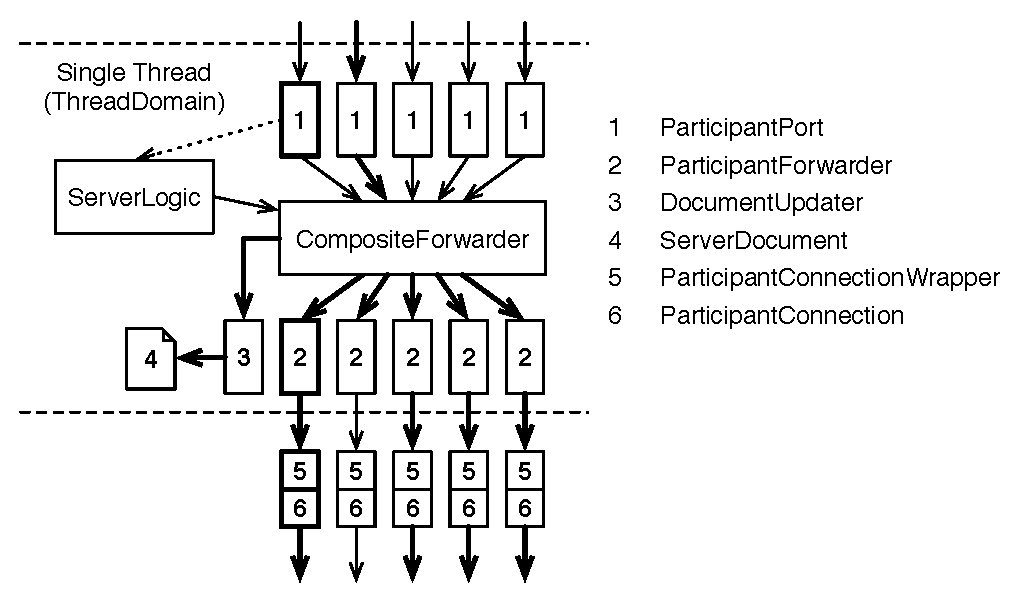
\includegraphics[width=16.9cm,height=9.67cm]{../images/finalreport/collaboration_serverflow.eps}
 \caption{Collaboration Layer Server}
 \label{fig:collaboration.serverflow}
\end{figure}

The server acts as a delivery station for messages from participants. 
Incoming requests are transformed by the corresponding 
\texttt{ParticipantPort} (1).
The resulting operation is passed to the \texttt{CompositeForwarder}, which in 
turn gives the request to all its child \texttt{Forwarders} (2 and 3). One child
forwarder is responsible to keep an up-to-date version of the document, whose
is named \texttt{DocumentUpdater} (3). The \texttt{DocumentUpdater} updates
a \texttt{ServerDocument} (4).

The other forwarders are \texttt{Participant\-Forwarder}s (2). They generate
requests, by using the server-side \texttt{Algorithm} for the corresponding
participant. The generated request is passed to a 
\texttt{Participant\-Connection\-Wrapper}, which forwards the request to
a target \texttt{Participant\-Connection}. The wrapper catches any exceptions
thrown by the target connection and notifies a \texttt{FailureHandler}
(not depicted in the figure \ref{fig:collaboration.serverflow}). The
\texttt{FailureHandler} is responsible to take the necessary actions in
case of a failure.

Objects assigned to the same participant are aligned vertically. So the
objects 1, 2, 5, and 6 that are aligned vertically belong all to the
same participant. One participant is the publisher of the document. In the 
figure it is the participant on the left.

The processing in the server from the point where a request crosses the
dashed line at the top to the point where all resulting requests have passed
the dashed line at the bottom must be sequential. This goal is achieved by
use of a \texttt{SingleThreadDomain} (see section 
\ref{sect:collaboration.threaddomains}).

\subsubsection{Example}
The bold arrows represent a request as it passes through the server. First,
it is received by the second \texttt{Participant\-Port} from the left. Then it 
is passed
to the \texttt{Composite\-Forwarder}, which forwards the request to all
its children. The \texttt{Participant\-Forwarder} (2) for the same 
participant filters the message. All the other \texttt{Forwarder}s pass the
message on to the \texttt{ParticipantConnectionWrapper} (5) (or to the
\texttt{ServerDocument} (4) in case of the \texttt{DocumentUpdater} (3)).


\subsection{Server Logic}
The \texttt{ServerLogic} provides methods that allows users to join,
participants leave, setting the document details, inviting users as well
as shutting down the server logic. So it provides the core methods
to manage the participants of a session. The interface is depicted in figure 
\ref{fig:collaboration.serverlogic}. 

\begin{figure}[H]
 \centering
 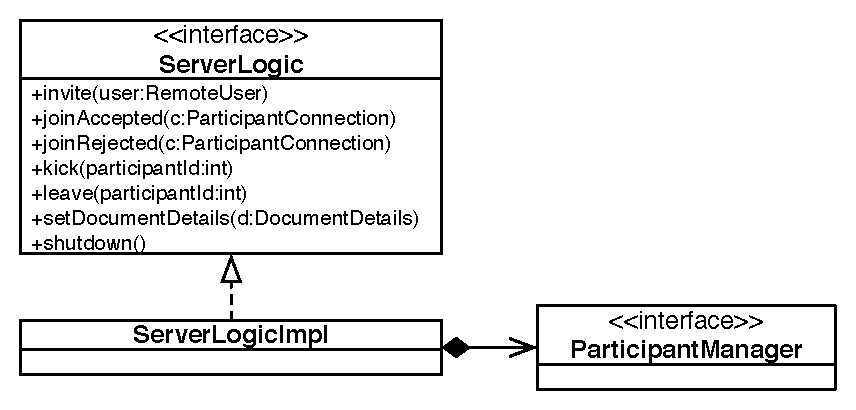
\includegraphics[width=13.93cm,height=6.39cm]{../images/finalreport/collaboration_serverlogic_uml.eps}
 \caption{ServerLogic Interface}
 \label{fig:collaboration.serverlogic}
\end{figure}

The \texttt{invite} method allows to invite a \texttt{RemoteUser} to
the session. The inherited \texttt{join} method from the
\texttt{DocumentServerLogic} interface allows the network layer to send
join requests. The \texttt{joinAccepted} and \texttt{joinRejected} methods
notify the logic that a join request was accepted or rejected. 

The \texttt{kick} method allows to kick the participant with the given
id to be kicked from the session. A kicked user is blacklisted, he
can no longer join the session. 

The \texttt{leave} notifies the
server logic that the participant identified by the given id left the
session. 

The \texttt{setDocumentDetails} method provides a way to change the
title of the document. This is used when the publisher saves the document
with a different name.

Finally, the \texttt{shutdown} method must be called when the session is
concealed by the publisher. It causes the server to properly dispose
all resources used by it.

\subsubsection{Participant Management}
The server logic implementation delegates the management of participants
to a class implementing the \texttt{ParticipantManager} interface. This
class is consulted to determine which users are currently in the
session (\texttt{isParticipant}), whether a user is blacklisted 
(\texttt{isBlacklisted}), whether the user has already sent a join
request which was not answered yet (\texttt{isJoining}), and whether a
user has been invited (\texttt{isInvited}).

\begin{figure}[H]
 \centering
 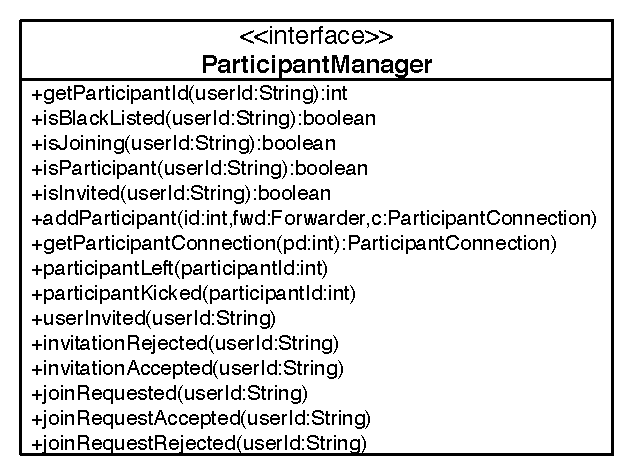
\includegraphics[width=10.16cm,height=7.48cm]{../images/finalreport/collaboration_participantmanager_uml.eps}
 \caption{ParticipantManager Interface}
 \label{fig:collaboration.participantmanager}
\end{figure}

The method \texttt{getParticipantId} is used to assign a user a participant
id. An implementation can assign a user that joins, leaves, and
rejoins the same session to assign the same participant id. The
\texttt{addParticipant} method is used to add a participant to the
session. The \texttt{getParticipantConnection} allows to get the 
\texttt{ParticipantConnection} for a participant.

The other methods exist to notify the \texttt{ParticipantManager} about
participant related events. An implementation of this interface can use
these methods to keep the internal data structures up-to-date. The
default implementation is \texttt{ParticipantManagerImpl}.


\subsection{Join Requests}
When a user tries to join, the request is encapsulated in an object
implementing the \texttt{Join\-Request} interface. The \texttt{Join\-Request}
is then passed to the publisher through the \texttt{Publisher\-Connection}.

The \texttt{Join\-Request} interface is
implemented by the \texttt{Join\-Request\-Impl} class. The implementation
is rather straightforward. The \texttt{accept}�method is passed to
the \texttt{join\-Accepted} method of the \texttt{Server\-Logic} interface.
The \texttt{reject} method is passed to the \texttt{join\-Requested}
method of the \texttt{Server\-Logic} interface.


\subsection{Participant Port}
Objects implementing the \texttt{ParticipantPort} interface are used 
by the network layer to pass messages from one participant to the
server logic (see figure \ref{fig:archoverview.participantport}). 
The implementation of that interface is 
\texttt{ParticipantPortImpl}. The participant port has a reference to
the server-side algorithm for the participant. Received requests are
transformed and then forwarded to a \texttt{Forwarder}.

The \texttt{leave} method of the \texttt{ParticipantPort} interface is
forwarded to the \texttt{leave} method on the \texttt{ServerLogic}. 

The port for a publisher is described later (see 
\ref{sect:archoverview.publisherport}).


\subsection{Forwarders}
We have already heard of the \texttt{CompositeForwarder} interface, which
represents a specialized version of the more general \texttt{Forwarder}
interface.

\begin{figure}[H]
 \centering
 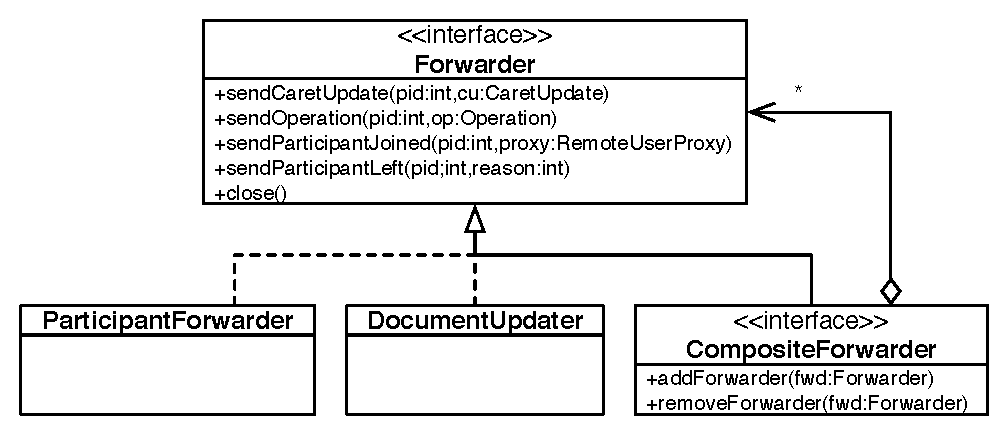
\includegraphics[width=16.51cm,height=6.81cm]{../images/finalreport/collaboration_forwarder_uml.eps}
 \caption{Forwarder inheritance hierarchy}
 \label{fig:collaboration.forwarder}
\end{figure}

A \texttt{Forwarder} is notified about certain events in the server. For
instance if a request from a participant is received, the transformed
operation is passed to the \texttt{sendOperation} method. Similar, there
is a \texttt{sendCaretUpdate} method for \texttt{CaretUpdate}s. Additionally
there are two methods that notify the \texttt{Forwarder} about participation
events. The \texttt{close} method is called when the \texttt{Forwarder}
is no longer needed.

\subsubsection{CompositeForwarder}
\label{sect:collaboration.compositeforwarder}
The \texttt{CompositeForwarder} is used by the implementation of the
server logic to send the events described above to a collection of
\texttt{Forwarder} objects. This interface adds methods to add and
remove \texttt{Forwarder} objects from the list of forwarders of the
\texttt{CompositeForwarder}. The only implementation of that
interface is \texttt{CompositeForwarderImpl}.

The \texttt{CompositeForwarderImpl} knows the concept of a default
forwarder. The default forwarder is a \texttt{Forwarder} that receives
all events as first forwarder. If the default forwarder throws an
exception, the event is not forwarded to the other forwarders. Instead
a \texttt{FailureHandler} is notified, which determines what to do
with that failure. The default forwarder used is described in 
section \ref{sect:archoverview.documentupdater}.

\subsubsection{ParticipantForwarder}
The \texttt{ParticipantForwarder} has a reference to the server-side algorithm
for one participant. There is a \texttt{ParticipantForwarder} for each
participant in the session. This type of forwarder generates requests for
the operations obtained through the \texttt{sendOperation} method and 
forwards them to the \texttt{ParticipantConnection} of that particular
participant. Similarly it generates a \texttt{CaretUpdateMessage} for
a \texttt{CaretUpdate}.

\begin{figure}[H]
 \centering
 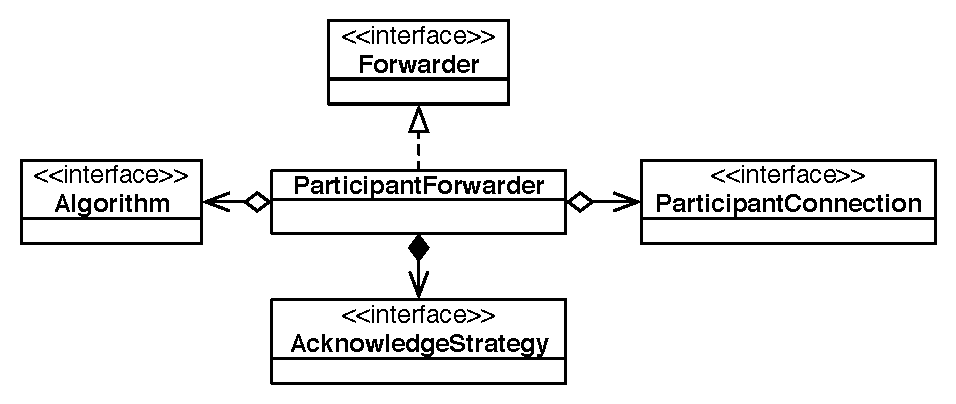
\includegraphics[width=15.63cm,height=6.28cm]{../images/finalreport/collaboration_participantforwarder_uml.eps}
 \caption{Forwarder for participants}
 \label{fig:collaboration.participantforwarder}
\end{figure}

The \texttt{ParticipantForwarder} gets a \texttt{AcknowledgeStrategy},
which is used to send acknowledge messages. See the section 
\ref{archoverview.acknowledgestrategies} for more information about
\texttt{AcknowledgeStrategy} objects.

\subsubsection{DocumentUpdater}
\label{sect:archoverview.documentupdater}
The last kind of \texttt{Forwarder} is a bit special. It is the
\texttt{DocumentUpdater}, which updates an object implementing the
\texttt{ServerDocument} interface. This is the server copy of the document,
which is sent to users that join the session. For more information see
the section \ref{sect:archoverview.serverdocument}.

\begin{figure}[H]
 \centering
 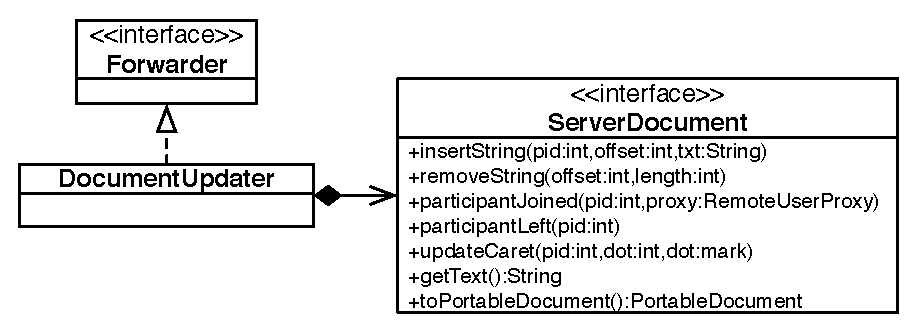
\includegraphics[width=15.00cm,height=5.08cm]{../images/finalreport/collaboration_documentupdater_uml.eps}
 \caption{DocumentUpdater and ServerDocument}
 \label{fig:collaboration.documentupdater}
\end{figure}

The \texttt{DocumentUpdater} is set as the default forwarder for the
\texttt{CompositeForwarderImpl}. This has an important implication. If the
\texttt{ServerDocument} does not accept the operation (e.g. if the insertion
index is wrong), the \texttt{FailureHandler} is notified. The default
implementation of the \texttt{FailureHandler} (the class 
\texttt{ServerLogicImpl}) removes the sender of the failing operation
from the session and notifies all the other participants that the participant
left (\texttt{sendParticipantLeft}).


\subsection{Server Document}
\label{sect:archoverview.serverdocument}
The \texttt{ServerDocument} is used by the server to keep an up-to-date
copy of the document that can be sent to users that want to join the
session. The class diagram of the \texttt{ServerDocument} can be found
in the section about the \texttt{DocumentUpdater} (see figure 
\ref{fig:collaboration.documentupdater}.

The \texttt{toPortableDocument} method creates a snapshot of the document
that can be sent to the \texttt{sendDocument} method of the 
\texttt{ParticipantConnection}. The other methods are used to update the
document.

The default implementation extends the \texttt{AbstractDocument} of Swing.
It uses the \texttt{Element} interface from Swing to model the fragments
of the document. Each continous block of text that belongs to the
same participant is an element. This element structure has to be kept
up-to-date if text is inserted and removed. The participant id of each
fragment is kept as an attribute in the \texttt{Element}'s 
\texttt{AttributeSet}.


\subsection{Failure Handling}
The \texttt{ServerLogic} needs a solid failure handling, otherwise it can
easily happen that the replicas start to diverge. The interface
\texttt{FailureHandler} is used to handle failures in the server logic. 

\begin{figure}[H]
 \centering
 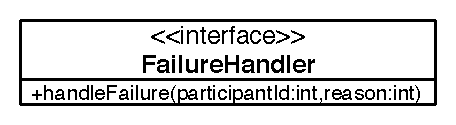
\includegraphics[width=7.16cm,height=1.55cm]{../images/finalreport/collaboration_failurehandler_uml.eps}
 \caption{FailureHandler Interface}
 \label{fig:collaboration.failurehandler}
\end{figure}

It is passed to all objects where errors can potentially occur. The failure
handler is passed to the following places.

\begin{itemize}
 \item participant ports
 \item \texttt{ParticipantConnectionWrapper}
 \item \texttt{CompositeForwarderImpl}
\end{itemize}

The \texttt{ServerLogicImpl} implements that interface. The 
\texttt{handleFailure} method has a participant id parameter. That parameter
is used to determine to which participant the failure is related. If
it is a normal participant, that participant is removed from the session
and all other participants are notified about the participant that left.

However, if the failing participant is the publisher, the session is
terminated. In the current implementation of ACE, the publisher is always
in the same Java Virtual Machine as the server logic. Thus, there should
never really be a failure. If there is, it is most likely a bug in the
implementation, from which we cannot recover.

\subsubsection{Participant Port Failures}
The participant ports transform incoming requests. If a request cannot
be transformed because it is invalid, the algorithm throws an exception.
This exception is caught by the participant ports and the participant
is expelled from the session. First, a participant that sends invalid requests
is not an acceptable participant, and second that particular participant
has an invalid document state. The operation has been applied locally but
the server rejected the corresponding request. Thus, the document state of
that particular participant starts to diverge from the correct document
content and so can no longer be part of the session.

\subsubsection{ParticipantConnectionWrapper}
The \texttt{ParticipantConnectionWrapper} wraps a \texttt{ParticipantConnection}
and catches exceptions thrown by the target connection. If the target throws
an exception, the \texttt{FailureHandler} is called.

A failing \texttt{ParticipantConnection} expells the concerned participant
from the session. More about the wrapper class can be read in the section
\ref{sect:collaboration.outgoingthreaddomain}.

\subsubsection{CompositeForwarderImpl}
The failure handling of the \texttt{CompositeForwarderImpl} is described
in detail in the section about composite forwarders (see section
\ref{sect:collaboration.compositeforwarder}).


\subsection{Usage of ThreadDomains}
\label{sect:collaboration.threaddomain}
The server logic uses \texttt{ThreadDomain}s extensively. To learn about
\texttt{ThreadDomain}s read the chapter \ref{chapter:threaddomains}.

\subsubsection{Outgoing ThreadDomain}
\label{sect:collaboration.outgoingthreaddomain}
The algorithm requires that the transformation of requests at the server
occurs sequentially. However, the sending of the resulting transformed
requests should occur in parallel. If the sending does not occur in parallel
then a slow connection could slow down the transformation throughput at
the server.

That is the reason why all the \texttt{ParticipantConnection}s are wrapped 
with a \texttt{ThreadDomain}. This has the disadvantage that exceptions
thrown by the target connection are not thrown back at the server logic.
In a similar way to the \texttt{SessionConnectionWrapper} the
\texttt{ParticipantConnectionWrapper} is used together with a
\texttt{FailureHandler} to handle failing connections. If a
\texttt{ParticipantConnectionWrapper} catches an exception thrown by the
target connection, the \texttt{FailureHandler} is notified and the
target connection is replaced with a null connection. The null connection
is a simple \texttt{ParticipantConnectionWrapper} that simple ignores
all method calls.

\begin{figure}[H]
 \centering
 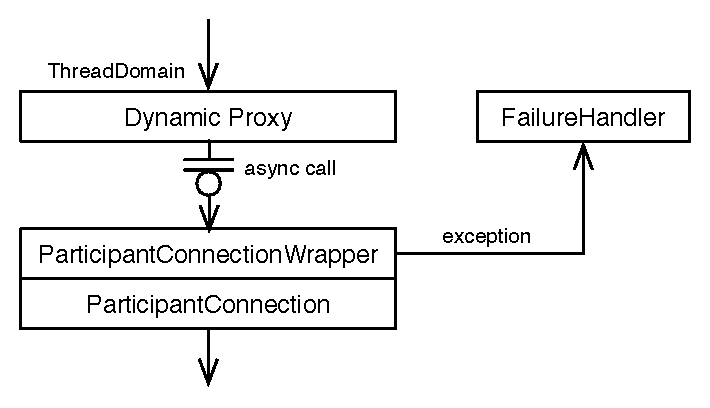
\includegraphics[width=11.47cm,6.35cm]{../images/finalreport/collaboration_participantconnectionwrapper.eps}
 \caption{Wrapped participant connection with ThreadDomains}
 \label{fig:collaboration.participantconnectionwrapper}
\end{figure}

The reason why we use these null connections is because the queues employed
by the thread domains might still contain method calls for that particular
connection. Instead of trying to remove those method invocations from the
queue, we simply ignore further calls.

There is also a \texttt{Publisher\-Connection\-Wrapper} that serves the same
purpose for \texttt{Publisher\-Connection} as the 
\texttt{Participant\-Connection\-Wrapper} serves for the
\texttt{Participant\-Connection}.

\subsubsection{Incoming ThreadDomain}
As noted above, only one thread may access the server logic transformation
section at any time. Now, instead of using synchronized statements or
locks, we use thread domains to ensure that only one thread accesses the
server logic at any given moment. How can this be achieved? By wrapping
all incoming references with a \texttt{SingleThreadDomain}. The possible
incoming references are:
\begin{itemize}
 \item all \texttt{ParticipantPort} instances
 \item \texttt{ServerLogic}
 \item \texttt{FailureHandler}
\end{itemize}

This technique allows to solve two problems: first, the transformation must
be serialized and second, the caller does not have to wait for the
transformation to be completed.

\subsubsection{Thread Domain in Server Logic}

% TODO: image with thread domains


\subsection{Hosting ServerLogic}
Nothing in the design of the whole server logic prevents it to be used outside
of ACE. All incoming requests pass through a \texttt{ParticipantPort}, all
outgoing through a \texttt{ParticipantConnection}. So the server logic
is totally agnostic about the fact that the publisher is running inside
the same Java Virtual Machine. So, through the introduction of few additional
interfaces it would be possible to host the server logic on a different
computer. This is not supported at the moment by ACE but it would be
a minor feature to implement the server part.



\section{Publisher}
The \texttt{ServerLogicImpl} class has a method 
\texttt{initPublisherConnection}. The parameter type of that method
is \texttt{PublisherConnection} and it returns an object implementing
\texttt{PublisherPort}.


\subsection{Publisher Connection}
% TODO: PublisherConnection

The \texttt{PublisherConnection} extends the \texttt{ParticipantConnection}
interface with methods that are only available for a connection to the
publisher. The \texttt{sessionFailed} method is called when there is
a serious error in the session logic, which does not allow any recovery.
The session is then no longer usable and the document no longer published.

The \texttt{sendJoinRequest} method sends a join request to the
publisher of the session.

The default implementation of the \texttt{PublisherConnection} interface
is the class \texttt{PublishedSessionImpl}. 


\subsection{Publisher Port}
\label{sect:archoverview.publisherport}
The interface \texttt{PublisherPort} extends the \texttt{ParticipantPort}
with methods only available to the publisher of the document. 

% TODO: PublisherPort

The \texttt{kick} method provides the publisher of the session a way to kick
one particular participant from the session. A kicked user is blacklisted
and no longer allowed to join the session (unless the publisher invites
him again).

The \texttt{invite} method is used to invite a user to the session and finally,
the \texttt{setDocumentDetails} method makes it possible to change the 
document title (for instance if the document is renamed).

The default implementation of the \texttt{PublisherPort} interface is
the \texttt{PublisherPortImpl} class.


\subsection{Published Session}
The publisher of a document gets a \texttt{PublishedSession} object from
the \texttt{publish} method of the \texttt{CollaborationService}. The
implementation of this interface is the \texttt{PublishedSessionImpl}
class, which, as we have seen, implements the \texttt{PublisherConnection}
interface too.

% TODO: PublishedSession, PublisherPort, Impl

The published session hosts the client-side algorithm of the publisher.
It also has a reference to a \texttt{AcknowledgeStrategy}, which is
used to send acknowledge strategies (see section 
\ref{sect:archoverview.acknowledgestrategies}).



\section{Miscellaneous}

\subsection{Acknowledge Strategies}
\label{sect:archoverview.acknowledgestrategies}
In the discussion of the algorithm (see section {sect:algorithm.outgoingqueue})
we have noted that
in some cases the outgoing queues of the \emph{Jupiter} algorithm can 
grow indefinitely. To avoid this situation, a site that does not generate
requests on its own but receives requests from the other site should acknowledge
from time to time the messages processed from the other site in order to 
avoid that the queues grow too much. Acknowledge messages are rather simple.
They must consist of the local site id as well as the local timestamp.

The collaboration layer uses objects implementing the 
\texttt{AcknowledgeStrategy} interface to determine when to send 
acknowledge messages. This is a classical implementation of the
\emph{Strategy} pattern. The strategy itself does not know how exactly to 
send an acknowledge message. This is left to an object implementing the
\texttt{AcknowledgeAction} interface, which has a single \texttt{execute}
method. That method is invoked by the strategy whenever it thinks it is
time to send an acknowledge message.

\begin{figure}[H]
 \centering
 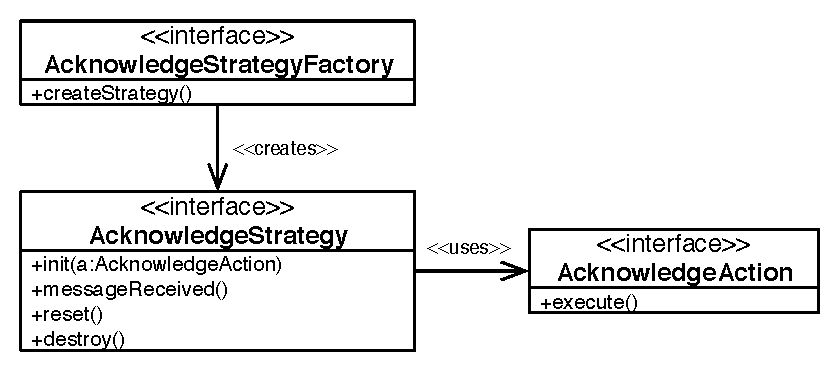
\includegraphics[width=13.65cm,height=5.72cm]{../images/finalreport/collaboration_acknowledge_uml.eps}
 \caption{AcknowledgeStrategy and related interfaces}
 \label{fig:collaboration.acknowledge}
\end{figure}

The strategies must be initialized with an action through the \texttt{init}
method. Code that uses an \texttt{AcknowledgeStrategy} should call
\texttt{reset} whenever a message with a timestamp in it is sent to the
other site. Such a message makes sending acknowledge messages useless, as the
sent message already contains a timestamp. If a message is received from
the other site, the \texttt{messageReceived} method should be called.

Acknowledge strategies can decide when it is time to send an acknowledge
message. A possible strategy is to send an acknowledge message back to the other
site whenever a certain number of messages have been received (this is
the strategy used by the \texttt{CountingAcknowledgeStrategy}). In that
case, the \texttt{reset} method resets the message counter to zero.

Another strategy could be based on a timer that fires after 60 seconds of
not sending any messages to the other site. The \texttt{reset} method in that
case would simple restart the timer.

The \texttt{AcknowledgeStrategyImpl} combines both strategies described
above. The timer is just started when there has been a received message.

ACE currently uses the simple message counting based implementation and not
the more complex and precise combined strategy. The timer based strategy
alone did not prove to be good enough, because potentially many messages
can be received in the timeout period.

\texttt{AcknowledgeStrategy} objects are creates by corresponding factories.
The factory interface is \texttt{AcknowledgeStrategyFactory}.





%%% Local Variables: 
%%% mode: latex
%%% TeX-master: "~/workspace/ace/www/"
%%% End: 
